\documentclass[12pt]{report}
\usepackage{mathptmx}
\usepackage[14pt]{moresize}
\usepackage{geometry}
\geometry{legalpaper, margin=1in}
%Margini e interlinea
\usepackage[top=1in, bottom=1in, left=1.4in, right=1in]{geometry}

\usepackage[italian]{babel}
\usepackage[utf8x]{inputenc}
\newcommand{\me}{\mathrm{e}}
\usepackage{amsmath}
\usepackage{tabularx}
\usepackage{setspace}
\usepackage{natbib}
\usepackage{multicol}
\usepackage{ragged2e}
\usepackage{graphicx}
\usepackage[toc,page]{appendix}
\usepackage[colorinlistoftodos]{todonotes}
\usepackage{subfig}
\usepackage{float}
\usepackage{floatrow}

\begin{document}

\begin{titlepage}

\newcommand{\HRule}{\rule{\linewidth}{0.5mm}} % Defines a new command for the horizontal lines, change thickness here

\center % Center everything on the page
 
%----------------------------------------------------------------------------------------
%	HEADING SECTIONS
%----------------------------------------------------------------------------------------

% Name of your university/college
\textsc{\Large \textbf{Parallel and distributed systems: paradigms and models \\}}\\[0.50cm]
\textsc{\Large \textbf{Academic Year 2018-2019 \\}}\\[0.75cm]
\textsc{\Large \textbf{Final project \\}}\\[0.75cm]

\textsc{\Large \textbf{\it{Autonomic farm pattern \\}}}\\[0.50cm]

{ \it \\[0.5cm]}{\\[0.5cm]\\[0.75cm]}\\[3.0cm]\textsc{\textbf{Luca Corbucci \\[0.35cm]Matricola: 516450}}\\[1cm] % Minor heading such as course title

%----------------------------------------------------------------------------------------
%	TITLE SECTION
%----------------------------------------------------------------------------------------


\includegraphics[width=2.5cm]{Stemma_unipi.png}\\[2cm]
 
%----------------------------------------------------------------------------------------
%	AUTHOR SECTION
%----------------------------------------------------------------------------------------
\textsc{Dipartimento di Informatica\\[0.15cm]\textsc{\textbf{Università di Pisa}}\\[0.05cm]\\[0.15cm]}{Settembre 2019}
% If you don't want a supervisor, uncomment the two lines below and remove the section above
%\Large \emph{Author:}\\
%John \textsc{Smith}\\[3cm] % Your name
\end{titlepage}
%----------------------------------------------------------------------------------------
%	DATE SECTION
%----------------------------------------------------------------------------------------

% Include a department/university logo - this will require the graphicx package

\newpage
\doublespacing\tableofcontents
\newpage
\chapter{Introduzione}

Il progetto consiste nello sviluppo di una farm capace di adattare autonomamente il numero di worker attivi in base ad un certo service time scelto dall'utente.\\L'autonomic farm viene avviata fornendo:
\begin{itemize}
\item Una collezione di task in input da calcolare;
\item Una funzione per calcolare ognuno dei task;
\item Il tsGoal atteso;
\item Un parallelism degree iniziale.
\end{itemize}\\Questo framework è stato implementato in C++ utilizzando i classici Thread e poi usando FastFlow.

\chapter{Analisi del problema}

L'implementazione dell'Autonomic Farm è simile a quella di una classica farm, ad esclusione del fatto che in questo caso è presente anche la possibilità di modificare il numero di worker attivi.
La modifica del numero dei worker deve permettere di mantenere durante tutta l'esecuzione dell'Autonomic Farm Pattern un service time prossimo a quello indicato come parametro. Idealmente vorremmo ottenere un grafico della variazione del service time simile a quello della figura \ref{Ideal} con degli aumenti e delle diminuzioni del valore dovuti alla variazione di task che deve essere calcolato.

\begin{figure}[H]
\centering
  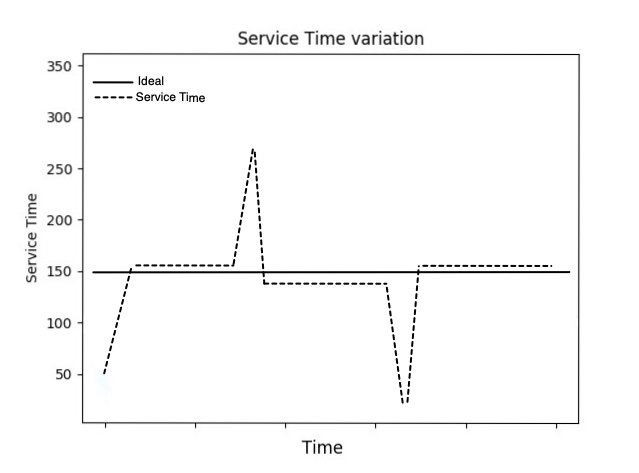
\includegraphics[width=0.7\linewidth]{IdealTS.jpg}
  \caption{Variazione ideale del service time, in corrispondenza della variazione del task il service time aumenta o diminuisce, poi viene riportato al valore ideale modificando il numero di worker attivi}
  \label{Ideal}
\end{figure}

L'idea è stata quella di creare vari componenti andandoli poi ad unire in modo da formare l'Autonomic Farm.
Nel caso dell'implementazione con i thread di C++ abbiamo i seguenti componenti:

\begin{itemize}
\item Emitter
\item Worker
\item Collector
\end{itemize}

\begin{figure}[H]
\centering
  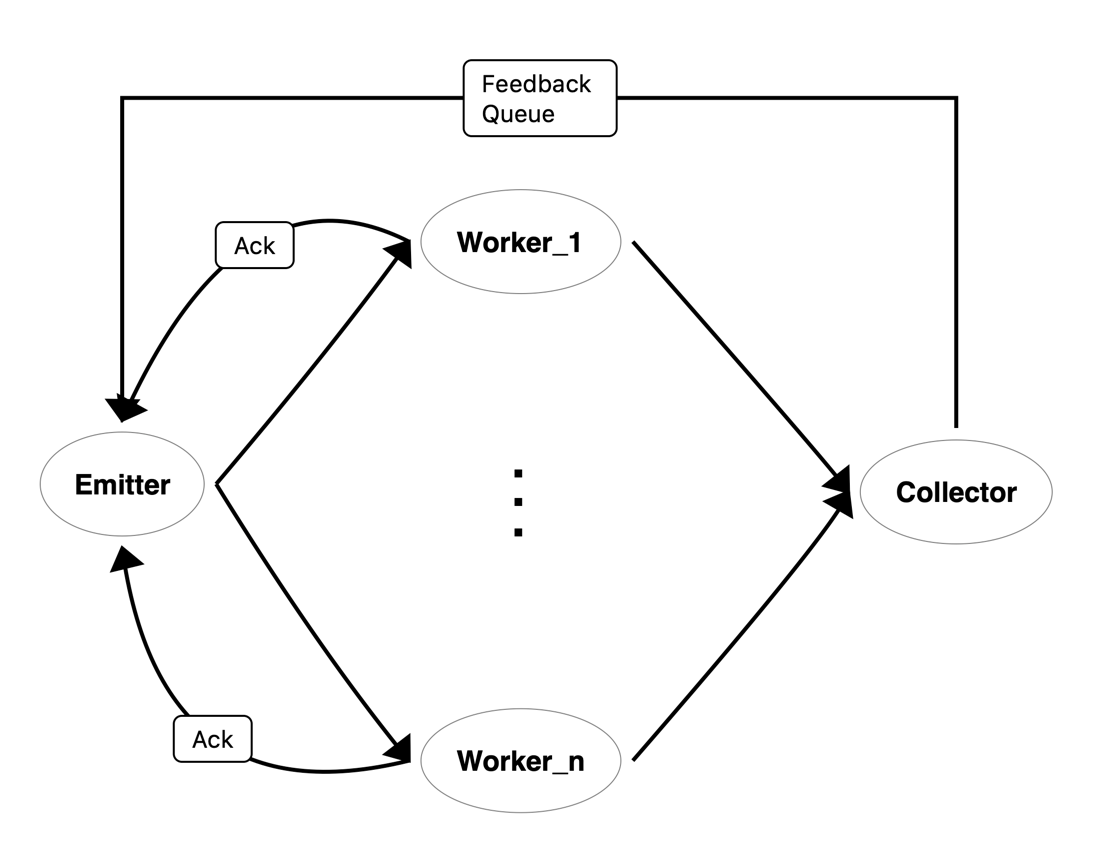
\includegraphics[width=0.7\linewidth]{ClassicThreads.png}
  \caption{Organizzazione dei componenti nell'implementazione ``Classic Threads"}
  \label{}
\end{figure}



Nel caso di FastFlow invece abbiamo:
\begin{itemize}
\item Emitter
\item External Emitter
\item Worker
\item Collector
\end{itemize}

\begin{figure}[H]
\centering
  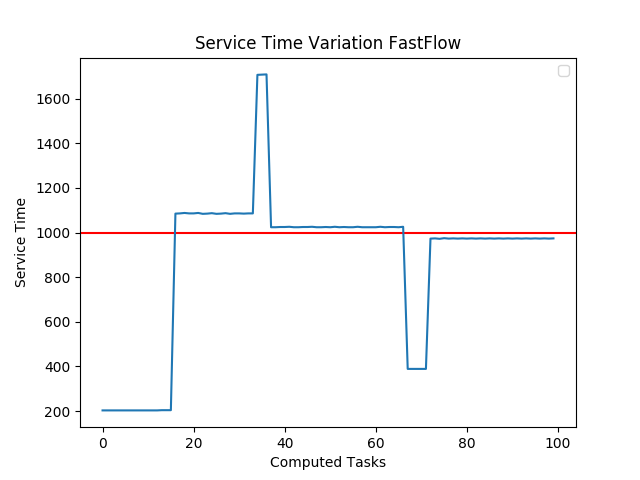
\includegraphics[width=0.7\linewidth]{FastFlow.png}
  \caption{Organizzazione dei componenti nell'implementazione con FastFlow.}
  \label{FastFlowComponents}
\end{figure} 
Rispetto alla soluzione con i thread classici, nella versione implementata con FastFlow è stato necessario creare un componente in più, chiamato External Emitter.
Nel caso di FastFlow il progetto è stato implementato utilizzando una pipeline che contiene come primo componente l'external emitter e come secondo componente la farm.
Questa scelta è stata necessaria per fare in modo che l'emitter possa ricevere tutti i vari task da eseguire inoltrandoli immediatamente ad un worker (se disponibile) oppure memorizzandoli in un array.
I task memorizzati nell'array verranno inoltrati ad un worker nel momento in cui questo invierà un ack all'emitter per notificare la terminazione della computazione che gli era stata precedentemente assegnata.

\chapter{Struttura del progetto e documentazione}

Il pacchetto contenente il progetto è organizzato nelle seguenti cartelle:
\begin{itemize}
\item src: contiene tutto il codice che è stato prodotto. All'interno della cartella src sono presenti varie sotto cartelle:
\begin{itemize}
\item AFP-FFQueue: contiene l'implementazione dell'Autonomic Farm che utilizza le code di FastFlow per la comunicazione;
\item AFP-SafeQueue: contiene l'implementazione dell'Autonomic Farm che utilizza le code con le lock per la comunicazione; 
\item FastFlow: implementazione dell'autonomic farm utilizzando FastFlow;
\item Utils: vari file e librerie utilizzate all'interno del progetto;
\item Test: contiene il makefile e i file di test che ho usato per provare l'autonomic farm.
\end{itemize}
\item Lib: contiene i file di FastFlow;
\item Doc: documentazione del progetto;
\item Report: contiene il report del progetto.
\end{itemize}\\Tutto il codice è stato commentato in modo da rendere chiaro il funzionamento, inoltre ho utilizzato Doxygen per generare la documentazione del progetto.

\chapter{Scelte implementative}

\section{Funzionamento Emitter}

L'emitter deve gestire la modifica del numero di worker attualmente attivi, per farlo memorizza due array di lunghezza pari al numero di worker:
\begin{itemize}
\item Il primo array serve per memorizzare se un worker è attualmente impegnato nel calcolo di un task o se è libero
\item Un secondo array serve per memorizzare se un worker è stato addormentato o no
\end{itemize}\\Quando viene avviato per la prima volta l'emitter invia un task da completare a ciascuno dei worker che sono stati attivati, poi, una volta ricevuto il feedback deve addormentarne o risvegliarne alcuni (nella sezione dedicata ai worker verrà spiegato come vengono addormentati o risvegliati).
Quando l'emitter risveglia o addormenta un worker, modifica l'array di bit nella posizione corrispondente a quello specifico worker.
L'emitter invia un segnale anche se il worker da addormentare sta ancora eseguendo un precedente task. Sarà poi compito del worker terminare il lavoro che aveva iniziato e non fare altro fino a nuovo avviso.\\Una volta eseguita una modifica del numero di worker l'emitter attende un certo tempo (specificato come parametro dall'utente) per effettuare la modifica successiva. \\L'emitter ha i seguenti canali di comunicazione con l'esterno:
\begin{itemize}
\item Un numero di code pari al numero di worker per inviare i task ai vari worker;
\item Una coda per ricevere gli ack dai vari worker in modo da capire quando finisce il lavoro;
\item Una coda per ricevere il feedback dal collector.
\end{itemize}\\Quando l'emitter ha terminato il suo lavoro, risveglia tutti i worker e poi invia un task ``speciale'' (contenente una variabile con valore ``-1") in modo che anche questi possano terminare.

\section{Funzionamento Worker}

Ogni worker svolge i seguenti passaggi:
\begin{itemize}
\item Riceve un task dall'emitter;
\item Calcola quel task memorizzando il tempo prima dell'inizio della computazione e il tempo finale;
\item Invia al collector il risultato della computazione effettuata.
\end{itemize}\\Il worker deve essere in grado di fermarsi su richiesta dell'emitter, per questo al suo interno ha una variabile di condizione che viene utilizzata per eseguire la wait() e poi per risvegliare il thread.
Sono stati implementati due metodi che possono essere chiamati dall'emitter:
\begin{itemize}
\item stopWorker(): metodo che setta a false un booleano ``status", quando il worker termina la computazione del task che ha ha ricevuto in precedenza, controlla se questo booleano è false e in tal caso esegue la wait su una variabile di condizione;
\item restartWorker(): metodo che modifica il valore del booleano ``status'' ed esegue una $notify\_one()$ sulla variabile di condizione, in questo modo il worker può risvegliarsi e può eseguire la computazione del prossimo task.
\end{itemize}

\section{Funzionamento Collector}

Il collector si occupa di gestire il calcolo del numero di worker che dovranno essere mantenuti attivi per garantire il service time che abbiamo scelto di avere.
In particolare per calcolare quanti worker dovranno svolgere i task successivi ho utilizzato questa formula:

\begin{equation}
    Nuovo \ Numero \ Worker = \frac{Tempo \ computazione \ di \ un \ task}{TSGoal}
\end{equation} \\Una volta calcolato il nuovo numero di worker, il collector utilizza la feedback queue che lo collega all'emitter per inviare questa informazione.
Sarà poi l'emitter a inviare i segnali ai vari worker per fare in modo che questi vengano addormentati o risvegliati.\\Il collector ha anche il compito di memorizzare in una coda il risultato dell'esecuzione della funzione calcolata nel worker. Opzionalmente questa coda di risultati può anche essere stampata.

\section{Comunicazione tra emitter, worker e collector}

Quando ho iniziato il progetto una delle prime cose che ho fatto è stata un'implementazione della farm che però non comprendeva ancora la possibilità di modificare il numero di worker. 
In questo primo test avevo utilizzato per la comunicazione tra l'emitter e i vari worker e tra i worker e il collector, delle code ``Safe'' implementate utilizzando le lock.
L'utilizzo di queste code e di Task abbastanza semplici da far svolgere al Worker mi hanno portato a pensare che non fosse corretto sfruttarle nel progetto perchè il tempo per la comunicazione risultava essere maggiore rispetto al tempo necessario per svolgere il task.
Quindi ho provato una soluzione differente ed ho utilizzato le code senza lock di FastFlow.\\Una volta completata l'implementazione dell'Autonomic Farm pattern ho confrontato le prestazioni dei due sistemi di comunicazione e ho avuto due risultati differenti dipendenti dal tipo di task eseguito:
\begin{itemize}
\item Facendo svolgere all'Autonomic Farm un task abbastanza ``pesante'' (ad esempio il calcolo della funzione di Fibonacci con un numero maggiore di 30), tra i due sistemi di comunicazione non sono presenti grandi differenti e il tempo di completamento è molto simile.
Il test in questione è stato svolto sullo Xeon Phi.
In questo test ho utilizzato 128 worker, un tsGoal pari a 15 e il task da calcolare era la funzione di Fibonacci, nella coda di input ho utilizzato tre valori differenti.
Il test può essere riprodotto eseguendo il file $testConfronti.sh$. Per ognuna delle opzioni sono stati eseguiti 5 test differenti in modo da calcolarne poi la media dei tempi di esecuzione, nella tabella \ref{tab:TableTaskPesante} è presente il risultato ottenuto, il tempo è espresso in secondi.

\begin{table}[H]
\begin{center}
\begin{tabular}[b]{cc}\hline
    Tipo Coda & Tempo\\
    \hline
    Safe Queue & 76,83s\\
    Code FastFlow & 76,46s\\ \hline
\end{tabular}
\end{center}

\caption{\label{tab:TableTaskPesante}Completion time dell'Autonomic Farm con task ``pesanti"}
\end{table}


I tempi riportati nella tabella prendono in considerazione la creazione di tutti i componenti necessari all'autonomic farm, la loro esecuzione e la successiva join.

\item Il discorso è decisamente differente se calcoliamo un task più ``semplice", ad esempio un controllo del numero primo o la funzione di Fibonacci con numeri piccoli.
In questo caso la differenza tra i due sistemi di comunicazione è piuttosto evidente, nella tabella \ref{tab:TableTaskLeggero} confrontiamo i tempi di completamento dello stesso test eseguito sullo Xeon Phi e sul mio computer (MacBook Pro con processore Intel i7 con 4 core e 8 contesti).
    \begin{table}[H]
    \begin{center}
    \begin{tabular}[b]{cccc}\hline
    Task & Macchina & Tempo Safe Queue & Tempo Coda FastFlow\\ \hline
    Fibonacci & XeonPhi & 23.22s & 2.64s\\
    Fibonacci & MacBook & 13.77s & 0.72s\\
    isPrime & XeonPhi & 242.67 & 20.15\\
    isPrime & MacBook & 157.19 & 7.14\\
    \hline
    \end{tabular}
    \end{center}
    
    \caption{\label{tab:TableTaskLeggero} Confronto tra i completion Time dell'Autonomic Farm con Safe Queue e code di FastFlow con task ``leggeri"}
    \end{table}
\end{itemize}\\La mia impressione è che utilizzando task più pesanti si riesca a mascherare meglio il tempo della comunicazione mentre con task ``semplici'' questo risulta dominante rispetto al tempo della computazione.\\Per cercare di capire meglio il funzionamento delle due implementazioni ho utilizzato Gprof, all'interno della cartella Test sono presenti i risultati ottenuti con questa analisi (Analysis1.txt, Analysis2.txt, Analysis3.txt, Analysis4.txt).
L'analisi effettuata con Gprof ha evidenziato che nel caso dell'utilizzo delle Safe Queue e di un task veloce da calcolare, il 77\% del tempo della computazione viene speso per la comunicazione, quindi per il passaggio dei task da emitter a worker e soprattutto per l'invio dei feedback dal collector all'emitter.
La stessa cosa non accade utilizzando le code di FastFlow e  task ``semplici", in questo caso il 94\% del tempo complessivo viene speso per il calcolo della funzione dei workers.
La situazione è differente quando andiamo ad utilizzare task più pesanti che quindi richiedono più tempo per essere calcolati. In questo secondo caso Gprof indica che i tempi necessari per il calcolo della funzione sono dominanti rispetto a tutto il resto, sia utilizzando le Safe Queue sia le code di FastFlow.

\section{Opzioni}

I file che ho creato per testare il progetto possono essere eseguiti indicando dei parametri e delle opzioni da cui dipende il comportamento del programma.\\Le opzioni sono state implementate utilizzando la libreria cxxopts.hpp \cite{cxxopts}, quelle che ho scelto di inserire sono le seguenti:

\begin{itemize}
\item -s: va utilizzata specificando un valore true o false, serve per indicare l'utilizzo o meno della safe queue;
\item -f: serve per indicare l'utilizzo dell'Autonomic Farm implementata con FastFlow, va usato senza specificare l'opzione precedente;
\item -d: opzione di debug usata per stampare alcune statistiche e informazioni generate dall'autonomic farm pattern.
\end{itemize}

\chapter{Benchmark}

Gli esperimenti sono stati eseguiti sulla CPU Xeon Phi con 64 core fisici, ognuno dei quali ha 4 contesti.
Nei seguenti paragrafi ogni tempo è espresso in millisecondi e rappresenta la media di 5 test differenti svolti sulla stessa macchina e con gli stessi parametri.
Ognuna delle soluzioni implementata è stata testata con un numero di thread attivi $N \in {1,2,...., 128}$.
Per eseguire l'autonomic farm pattern è possibile utilizzare uno dei test presenti nella cartella ``Test'' specificando i seguenti parametri:
\begin{itemize}
\item Numero di worker;
\item TSGoal;
\item Dimensione della collezione in input;
\item Valore in input nella prima parte della collezione;
\item Valore in input nella seconda parte della collezione;
\item Valore in input nella terza parte della collezione;
\item Valore intero che indica ogni quanto tempo vogliamo modificare il numero di worker.
\end{itemize}\\Tra i vari test è presente anche $testLeaks.sh$ che controlla se alla fine dell'esecuzione del programma è stata liberata o meno tutta la memoria precedentemente allocata.

\newpage
\section{Speedup}

La speedup è calcolata come $S(N) = T_{seq}/T_{par}(N)$.

\begin{figure}[H]
\centering
  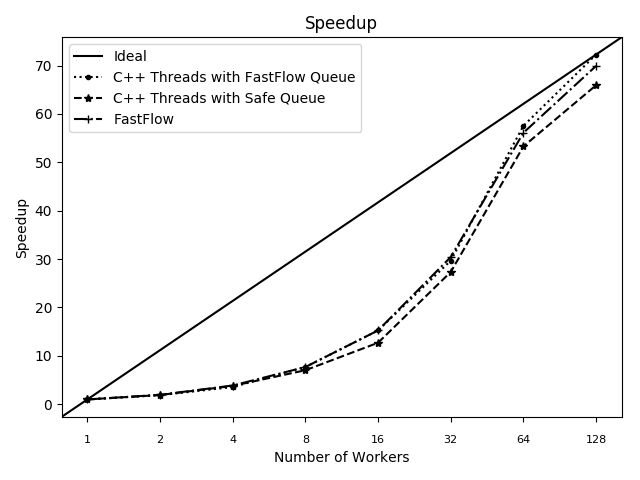
\includegraphics[width=0.65\linewidth]{Speedup.png}
  \caption{Speedup al variare del numero di worker e al tipo di implementazione}
  \label{Speedup}
\end{figure}

Nel grafico \ref{Speedup} è riportata la curva della speedup al variare del tipo di implementazione utilizzata (FastFlow/Classic Threads) e del tipo di comunicazione utilizzata (Safe Queue/FastFlow queue).
Dal grafico possiamo notare come la curva della speedup inizia a rallentare a partire da $N=64$.

\section{Scalability}

La scalability è calcolata come $Scalability(p)=T_{par}(1)/T_{par}(N)$.
Per il calcolo della scalability ho eseguito un test sullo Xeon Phi.
Il test può essere replicato eseguendo il seguente comando:
$testScalability.sh$.\\Nel grafico \ref{Scalability} viene mostrata la curva della scalability.

\begin{figure}[H]
    \centering
    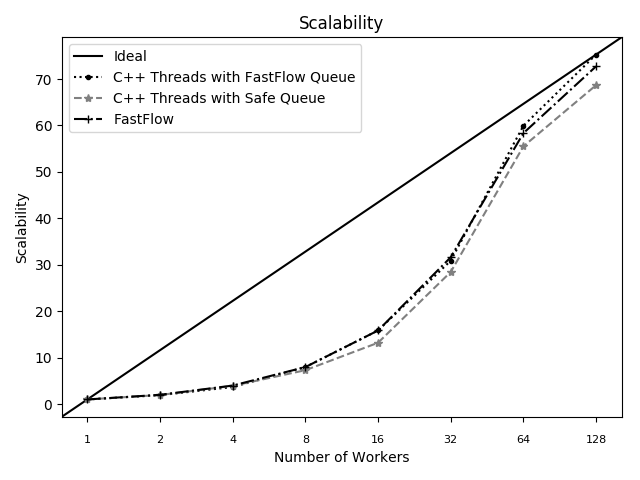
\includegraphics[width=0.65\linewidth]{Scalability.png}
    \caption{Grafico dell'andamento della Scalability}
    \label{Scalability}
  \end{figure}


\section{Completion Time}

Per confrontare i tempi di completamento ho effettuato il seguente test andando a variare il numero di thread utilizzati, ho replicato ogni esperimento per 5 volte e i dati riportati sono una media dei risultati ottenuti.
Il test può essere replicato eseguendo $testCompletionTime.sh$.
Nel grafico \ref{CompletionTime} viene riportato il confronto del completion time tra le varie implementazioni dell'Autonomic Farm, nella tabella \ref{tab:TableCompletionTime} sono indicati i tempi delle esecuzioni del test eseguito sullo Xeon Phi.

\begin{figure}[H]
\centering
  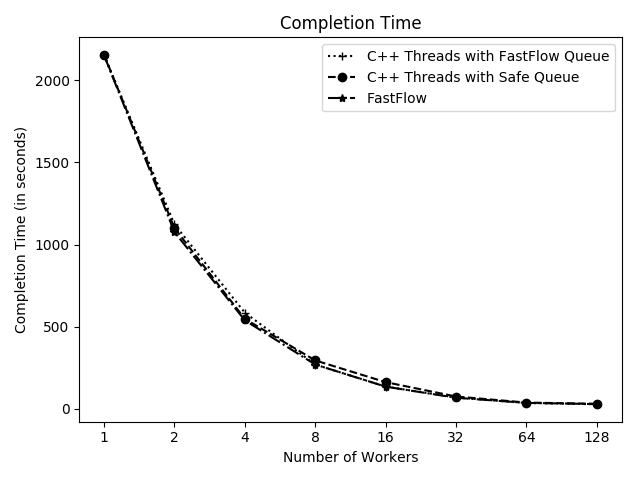
\includegraphics[width=0.8\linewidth]{Completion_Time.png}
  \caption{Completion time al variare del numero di workers e del tipo di implementazione utilizzata, il tempo è espresso in secondi}
  \label{CompletionTime}
  
\end{figure}


\begin{table}[H]
\begin{center}
\begin{tabular}[b]{cccc}\hline
      Worker & Tempo Safe Queue & Tempo FastFlow Queue & FastFlow \\ \hline
        1   & 2154.43s & 2154.31s & 2151.47s\\
        2   & 1099.97s & 1123.07s & 1076.60s\\
        4   & 548.22s  & 585.63s  & 539.22s\\
        8   & 295.27s  & 270.16s  & 270.09s\\
        16  & 163.06s  & 135.84s  & 135.78s\\
        32  & 75.72s   & 69.76s   & 68.04s\\
        64  & 38.82s   & 35.95s   & 36.87s\\
        128 & 31.37s   & 28.62s   & 29.58s\\ \hline
\end{tabular}
\end{center}

\caption{\label{tab:TableCompletionTime} Completion time al variare del numero di workers e del tipo di implementazione utilizzata, il tempo è espresso in secondi}
\end{table}
\newpage
\section{Efficiency}

L'efficiency è calcolata come $E(n)\ =\ Tseq/(n*T(n))\ =\ Sp(n)/n$.

\begin{figure}[H]
    \centering
    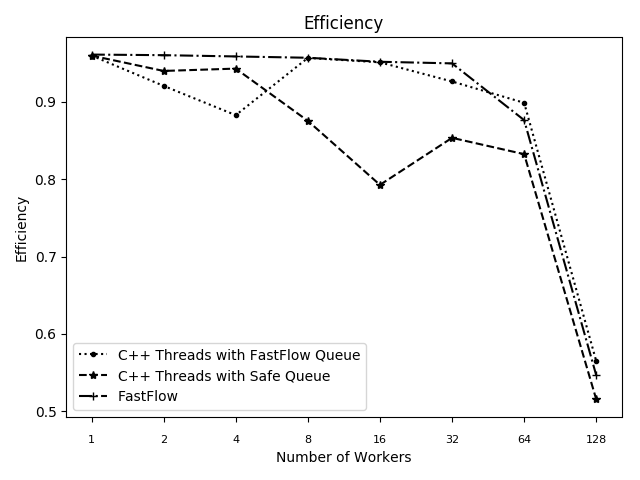
\includegraphics[width=0.65\linewidth]{Efficiency.png}
    \caption{Grafico dell'andamento dell'efficiency}
    \label{Efficiency}
  \end{figure}
  
Come possiamo vedere nel grafico \ref{Efficiency}, l'efficiency mantiene un valore prossimo allo $0.9$ fino a $N=64$ per poi scendere ad un valore vicino a $0.5$ nel momento in cui il numero di worker sale a 128.


\section{Variazione del Service Time}

Per capire la variazione del service time in base al numero di worker attivi e per comprendere quanto questo valore si distacca dal TsGoal passato come parametro all'Autonomic Farm ho pensato di produrre il grafico di Figura \ref{fig:TSVariationOnlyTS} che mostra l'andamento del valore del Service Time:

\begin{figure}[H]
\centering
  \subfloat[Andamento del service Time con 64 thread e un tTsGoal uguale a 100]{\label{fig:TSVariationOnlyTS}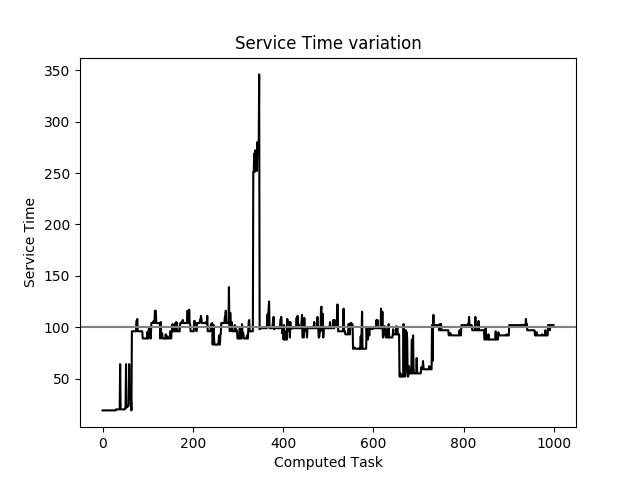
\includegraphics[width=0.5\linewidth]{ServiceTimeVariation_OnlyTS.png}}
  \subfloat[Andamento del service Time e confronto con la variazione del numero di workers]{\label{fig:TSVariationFULL}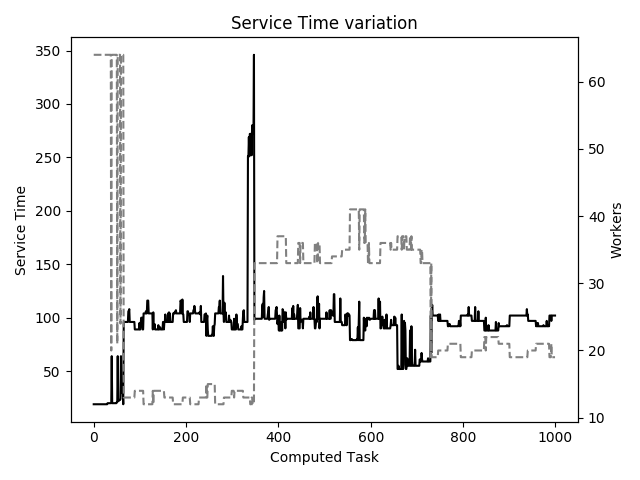
\includegraphics[width=0.5\linewidth]{ServiceTimeVariation_Full.png}}
  \caption{}
\end{figure}


L'esperimento è replicabile con il seguente comando:
$mainFib.out\ 64\ 100\ 1000\ 39\ 41\ 40\ 1500\ -d\ ts$.
Gli aumenti improvvisi del service time che vediamo nel grafico sono dovuti al fatto che in quel momento si inizia a lavorare su un task differente rispetto al precedente e quindi la farm deve adattarsi e modificare il numero di worker in modo da ottenere il service time desiderato.
Dalla figura \ref{fig:TSVariationFULL} possiamo notare come in corrispondenza di un aumento del service time (riga nera) ci sia anche una modifica del numero di worker (riga tratteggiata) che permette di riportare il service time al valore passato come parametro.\\In questo caso è stata eseguita l'Autonomic Farm con 64 thread, un TsGoal pari a 100ms, 1000 task in input e un aggiornamento del numero di worker ogni secondo e mezzo.
Il service time in questo caso ha assunto in media un valore pari a 92.

\chapter{Conclusioni}

Guardando i dati relativi alla Scalability e allo Speedup possiamo vedere come l'implementazione con i thread di C++ e l'utilizzo delle code di FastFlow ci fornisca un risultato di poco migliore rispetto alle altre soluzioni. 
L'utilizzo delle code di FastFlow ci permette di avere buone prestazioni indipendentemente dal task che vogliamo far calcolare ai worker, a differenza della soluzione con le Safe Queue che non ci garantisce un tempo di completamento accettabile quando utilizziamo dei task ``semplici''.
Dal punto di vista del programmatore che produce il framework la soluzione migliore è quella che sfrutta FastFlow perchè risulta più semplice implementare il tutto.

\newpage
\bibliographystyle{unsrt}
\bibliography{references}


\end{document}